%=====================================================================
\section{The data}
\label{sec:data}

The instances are the \textbf{EV-Solomon} set: the 56 Solomon routing files, read as EV-charging instances, at
sizes $n=10,20,\dots,100$ --- $56\times10=560$ instances. Timing is exactly Solomon's (the request is the
``ready time'', the deadline $T$ the depot due date, one grid unit one minute); within a Solomon class the
instances differ only in which cars request when. Each station has 2 guns of 22\,kW, and there are 5 vans.

Onto every EV two attributes are placed, the same number keeping the same pair across a class. The share of
\emph{commercial} cars and the two income distributions are calibrated from Indian data (about \fcomShareData\,\%
commercial among public-charging requests; income drawn from a Beta per segment --- personal skewed rich,
commercial skewed poor). Figure~\ref{fig:data} shows the result.

\begin{figure}[H]
\centering
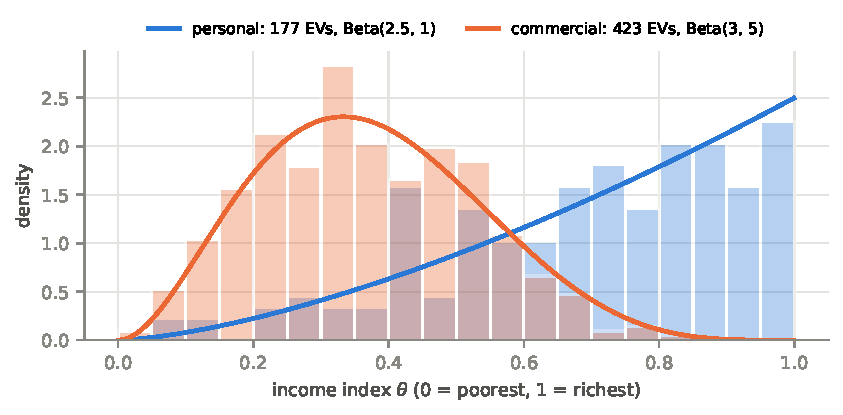
\includegraphics[width=0.82\textwidth]{figures/data_theta.pdf}\\[4pt]
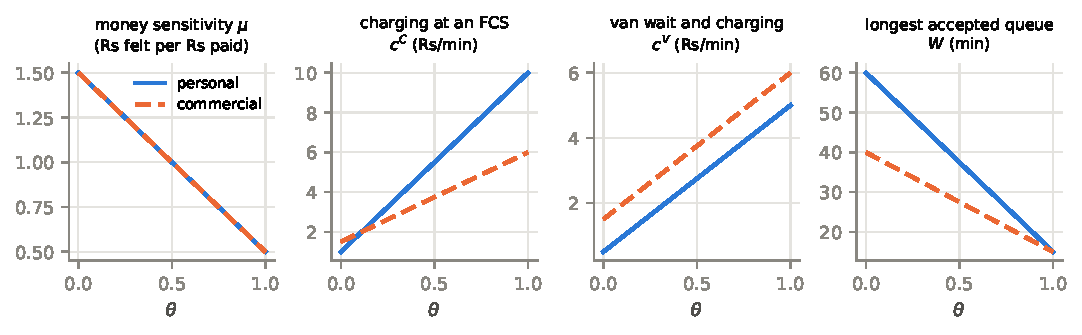
\includegraphics[width=\textwidth]{figures/data_lines.pdf}
\caption{Top: income $\theta$ of the EVs, personal (rich-skewed) and commercial (poor-skewed), with the
calibrated Beta densities. Bottom: how the coefficients move with income --- money felt falls, the value of
station and van time rises, the accepted queue falls; the two segments have different slopes and levels.}
\label{fig:data}
\end{figure}

\begin{table}[H]
\centering
\caption{The six Solomon classes as EV-charging instances (one file per class shown; shared within a class).}
\footnotesize
\begin{adjustbox}{max width=\linewidth}
\begin{tabular}{@{}lrrrrrrrrrr@{}}
\toprule
class & files & $T$ (min) & \shortstack{requests\\at 0 (\%)} & \shortstack{median\\$r/T$ (\%)} & \shortstack{mean $E$\\(kWh)} & \shortstack{stranded\\(\%)} & \shortstack{km to\\nearest FCS} & \shortstack{commercial\\(\%)} & \shortstack{mean $\theta$\\pers.} & \shortstack{mean $\theta$\\comm.} \\
\midrule
C1 & 9 & 1236 & 17 & 22 & 20.5 & 15 & 1.1 & 73 & 0.70 & 0.37 \\
C2 & 8 & 3390 & 19 & 29 & 20.5 & 15 & 1.6 & 69 & 0.72 & 0.39 \\
R1 & 12 & 230 & 25 & 23 & 18.3 & 15 & 1.9 & 70 & 0.64 & 0.37 \\
R2 & 11 & 1000 & 27 & 18 & 18.3 & 15 & 1.9 & 72 & 0.69 & 0.36 \\
RC1 & 8 & 240 & 19 & 25 & 19.9 & 15 & 1.8 & 66 & 0.73 & 0.35 \\
RC2 & 8 & 960 & 19 & 23 & 19.9 & 15 & 1.8 & 73 & 0.68 & 0.35 \\
\bottomrule
\end{tabular}
\end{adjustbox}

\end{table}

\inshort{560 Solomon-timed instances, 10--100 cars. Every car is tagged personal or commercial and given an
income, calibrated so that most public-charging demand is commercial and lower-income --- which is what makes the
segment the decisive variable.}

%=====================================================================
\section{Baseline --- the exact method (MILP)}
\label{sec:basemilp}

\begin{figure}[H]
\centering
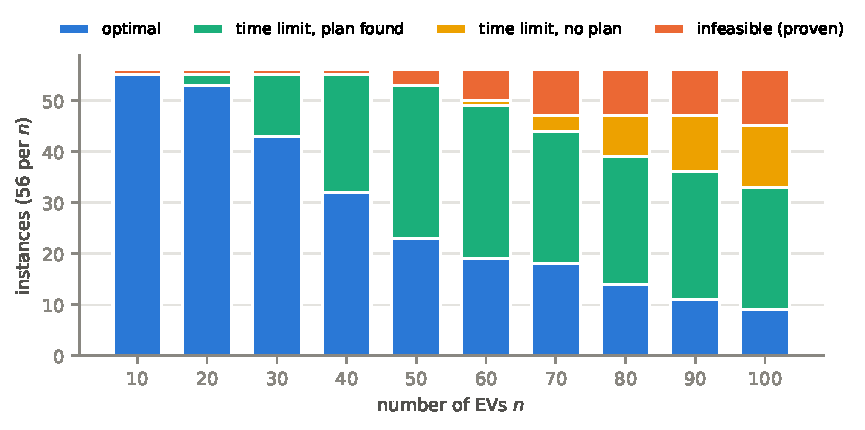
\includegraphics[width=0.86\textwidth]{figures/milp_status_by_n.pdf}
\caption{How the 560 baseline instances ended, by size (56 per size).}
\label{fig:milpstatus}
\end{figure}

\begin{table}[H]
\centering
\caption{MILP baseline by Solomon class. Median gap over the time-limited instances with a plan.}
\small
\begin{adjustbox}{max width=\linewidth}
\begin{tabular}{@{}lrrrrrrrrr@{}}
\toprule
class & instances & optimal & time limit & no plan & infeasible & valid & \shortstack{median\\gap (\%)} & \shortstack{mean\\time (s)} & \shortstack{mean $Z$\\(Rs)} \\
\midrule
C1 & 90 & 66 & 23 & 1 & 0 & 89 & 4.1 & 110 & 47470 \\
C2 & 80 & 56 & 23 & 1 & 0 & 79 & 2.9 & 109 & 47996 \\
R1 & 120 & 41 & 34 & 16 & 29 & 75 & 4.4 & 137 & 32677 \\
R2 & 110 & 70 & 40 & 0 & 0 & 110 & 2.6 & 130 & 44782 \\
RC1 & 80 & 13 & 29 & 16 & 22 & 42 & 7.8 & 171 & 36587 \\
RC2 & 80 & 31 & 48 & 1 & 0 & 79 & 2.9 & 189 & 49691 \\
\bottomrule
\end{tabular}
\end{adjustbox}

\end{table}

\textbf{Result.} \fmilpOptimal{} instances are solved to proven optimality, and \fmilpValid{} have a valid plan
in all; the mean solve time is \fmilpSolveMean\,s. Small instances ($\le20$ cars) are optimal in seconds; from
about 50 cars most hit the 300-second limit. The failures are all in the short-period classes R1 and RC1 at
60--100 cars, where many cars requesting late simply cannot all be charged by $T$ --- the \fmilpInfeasible{}
infeasible instances are \emph{proven} infeasible and are exactly the same set as in formulation~3, so
infeasibility comes from the \emph{data} (time, range, fleet), not from the customer model.

\subsection{What the cost is made of}
\begin{table}[H]
\centering
\caption{The six parts of $Z$ over the valid MILP plans (mean per instance and share).}
\small
\begin{adjustbox}{max width=\linewidth}
\begin{tabular}{@{}lrr@{}}
\toprule
term & mean per instance (Rs) & share of $Z$ (\%) \\
\midrule
$Z_1$ EV driving (perceived) & 388 & 0.9 \\
$Z_2$ van driving & 1067 & 2.4 \\
$Z_3$ van dispatch & 3291 & 7.5 \\
$Z_4$ operator energy & 9204 & 20.9 \\
$Z_5$ tariff (perceived) & 17310 & 39.3 \\
$Z_6$ time (perceived) & 12739 & 29.0 \\
\midrule
$Z$ (all six) & 43999 & 100.0 \\
\bottomrule
\end{tabular}
\end{adjustbox}

\end{table}
The felt tariff $Z_5$ is the largest part (\fshareZFive\,\%) --- every car pays for its energy and most customers
are poor commercial drivers who feel each rupee strongly --- then felt time $Z_6$ (\fshareZSix\,\%) and the
operator's electricity $Z_4$ (\fshareZFour\,\%). Van driving and dispatch are small (\fshareZTwo\,\% and
\fshareZThree\,\%). This split is used later: it is \emph{why} the money-sensitivity and demand levers are the
largest (they scale $Z_5$), and why the van-fleet lever is small (it touches only $Z_2,Z_3$).

\subsection{Who gets a van --- the theory in the data}
\begin{table}[H]
\centering
\caption{The two segments in the baseline plans (MILP and RL). Free-choice cars have a station in range.}
\small
\begin{adjustbox}{max width=\linewidth}
\begin{tabular}{@{}lrrrr@{}}
\toprule
 & personal MILP & personal RL & commercial MILP & commercial RL \\
\midrule
EVs in valid plans & 7043 & 7768 & 16787 & 18282 \\
free-choice EVs & 6095 & 6727 & 14125 & 15418 \\
van share of free-choice EVs (\%) & 19.9 & 6.7 & 0.7 & 0.9 \\
mean $\theta$ & 0.69 & 0.69 & 0.36 & 0.36 \\
mean queue at FCS (min) & 0.41 & 0.79 & 1.58 & 3.36 \\
mean wait for a van (min) & 19.8 & 21.8 & 24.5 & 28.3 \\
mean drive to FCS (min) & 7.8 & 8.3 & 8.9 & 11.3 \\
mean time until charged (min) & 60.6 & 61.8 & 64.3 & 68.3 \\
mean money paid (Rs) & 352 & 332 & 335 & 337 \\
mean time cost (Rs) & 381 & 430 & 200 & 214 \\
mean perceived cost (Rs) & 662 & 699 & 582 & 597 \\
\bottomrule
\end{tabular}
\end{adjustbox}

\end{table}

\begin{figure}[H]
\centering
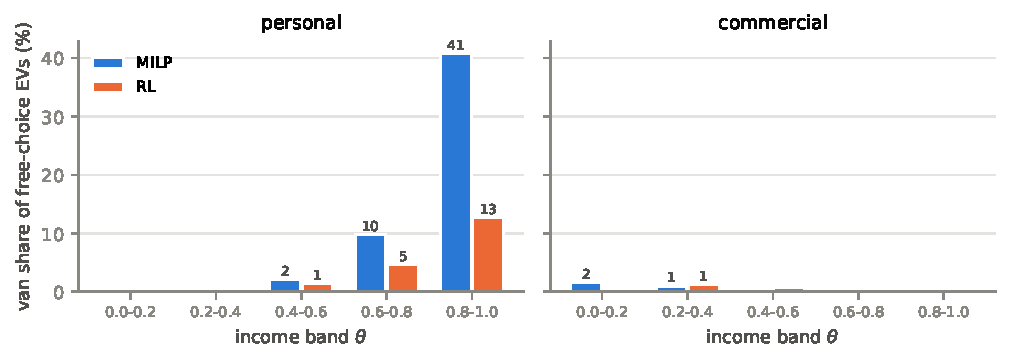
\includegraphics[width=0.95\textwidth]{figures/van_share_income.pdf}
\caption{Share of free-choice cars served by a van, by segment and income band.}
\label{fig:vanincome}
\end{figure}

\begin{table}[H]
\centering
\caption{By income band (MILP). ``Money felt'' is money paid times $\mu$.}
\footnotesize
\begin{adjustbox}{max width=\linewidth}
\begin{tabular}{@{}llrrrrrrr@{}}
\toprule
segment & \shortstack{$\theta$\\band} & EVs & van \% MILP & van \% RL & queue (min) & \shortstack{money\\felt (Rs)} & \shortstack{time cost\\(Rs)} & \shortstack{perceived\\cost (Rs)} \\
\midrule
personal & 0.0-0.2 & 125 & 0.0 & 0.0 & 1.45 & 389 & 120 & 509 \\
 & 0.2-0.4 & 690 & 0.0 & 0.0 & 1.32 & 403 & 243 & 646 \\
 & 0.4-0.6 & 1491 & 2.1 & 1.4 & 0.57 & 338 & 337 & 675 \\
 & 0.6-0.8 & 1934 & 9.8 & 4.7 & 0.18 & 263 & 428 & 691 \\
 & 0.8-1.0 & 2803 & 40.8 & 12.7 & 0.06 & 228 & 418 & 646 \\
\midrule
commercial & 0.0-0.2 & 2532 & 1.6 & 0.5 & 2.77 & 457 & 151 & 607 \\
 & 0.2-0.4 & 7633 & 1.0 & 1.3 & 1.76 & 408 & 186 & 594 \\
 & 0.4-0.6 & 5356 & 0.1 & 0.7 & 0.92 & 333 & 226 & 560 \\
 & 0.6-0.8 & 1186 & 0.0 & 0.5 & 0.75 & 286 & 273 & 559 \\
 & 0.8-1.0 & 80 & 0.0 & 0.0 & 0.00 & 167 & 258 & 425 \\
\bottomrule
\end{tabular}
\end{adjustbox}

\end{table}

The plans are a direct picture of the theory of Section~\ref{sec:theory}:
\begin{itemize}
  \item \textbf{Vans go to personal cars} (\fvanPersMilp\,\% of free-choice personal cars, \fvanComMilp\,\% of
  commercial) --- rule \textbf{(T1)}, the driver-free benefit is for private owners.
  \item \textbf{Among personal cars, van use climbs steeply with income} (0\,\% below $\theta=0.4$, about 41\,\%
  above 0.8); a logistic fit puts the personal threshold at $\theta^{*}\approx\fthetaStarPers$ --- rule
  \textbf{(T3)}.
  \item \textbf{The rare taxi with a van is a \emph{poor} driver with a long queue}, not a rich one --- rule
  \textbf{(T2)}: queues, not income, move taxis to vans. Commercial cars queue \fqueueComMilp{} min on average
  against \fqueuePersMilp{} for personal, so low-income customers absorb the congestion.
\end{itemize}

\support{The \fmilpInfeasible{} infeasible instances match formulation~3's exactly, so feasibility is a property
of the data; and the who-gets-vans pattern is the sign pattern of $\Delta_i$ in \eqref{eq:delP}--\eqref{eq:delC},
not a tuned outcome. The quantitative directions are checked against proven optima in Section~\ref{sec:validation}.}

\inshort{The MILP solves small instances exactly and large ones to within a few per cent; most of the cost is the
felt tariff and felt time; and the plans realise the theory --- vans for rich private owners, stations and queues
for taxis and the poor.}

%=====================================================================
\section{Baseline --- the learning method (RL)}
\label{sec:baserl}

\begin{table}[H]
\centering
\caption{RL against the MILP on the baseline, by class. Gap over instances valid in both.}
\small
\begin{adjustbox}{max width=\linewidth}
\begin{tabular}{@{}lrrrrrrr@{}}
\toprule
class & instances & MILP valid & RL valid & \shortstack{gap mean\\(\%)} & \shortstack{gap median\\(\%)} & MILP s & RL s \\
\midrule
C1 & 90 & 89 & 90 & 0.84 & 0.84 & 110 & 0.12 \\
C2 & 80 & 79 & 79 & 1.66 & 1.80 & 109 & 0.12 \\
R1 & 120 & 75 & 89 & 0.38 & 0.31 & 137 & 0.12 \\
R2 & 110 & 110 & 110 & 1.16 & 1.26 & 130 & 0.12 \\
RC1 & 80 & 42 & 52 & 0.12 & 0.33 & 171 & 0.12 \\
RC2 & 80 & 79 & 80 & 0.48 & 0.46 & 189 & 0.12 \\
\midrule
all & 560 & 474 & 500 & 0.85 & 0.76 & 140 & 0.12 \\
\bottomrule
\end{tabular}
\end{adjustbox}

\end{table}

\begin{figure}[H]
\centering
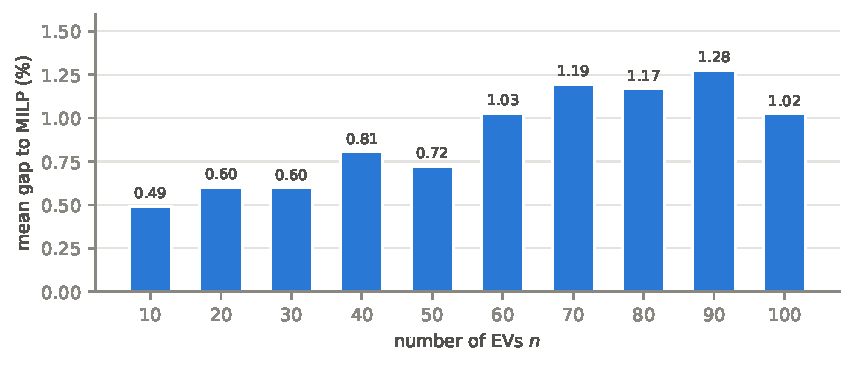
\includegraphics[width=0.82\textwidth]{figures/rl_gap_by_n.pdf}
\caption{Mean cost gap of the RL plan to the MILP, by instance size.}
\label{fig:rlgap}
\end{figure}

\textbf{Result.} The policy finds a valid plan in \frlValid{} instances (MILP \fmilpValid) --- including
\frlOnlyFromNoPlan{} where the MILP's 300-second search found none --- at a mean cost \frlGapMean\,\% above the
MILP (median \frlGapMedian\,\%), in \frlSolveMean\,s per instance against \fmilpSolveMean\,s. Its one weakness is
that it \emph{under-uses vans}: it gives vans to only \fvanPersRl\,\% of free-choice personal cars against the
MILP's \fvanPersMilp\,\%. So the RL cost and the \emph{direction} of its experiment effects are reliable, but its
van shares should not be read as the best policy --- for ``who gets a van'' the MILP is the reference.

\support{RL and the MILP are scored by the same checker (Section~\ref{sec:methods}), so the \frlGapMean\,\% is a
true quality gap, not a reporting artefact. That RL finds plans in \frlOnlyFromNoPlan{} instances the MILP could
not place within the time limit shows the two methods fail in different places, so agreement between them is
strong evidence. Section~\ref{sec:milpvsrl} shows the two methods give the \emph{same} experiment conclusions to
within about \fagreeRtMean{} percentage points.}

\inshort{RL is a fast, robust stand-in: valid plans in \frlValid{} instances, about \frlGapMean\,\% dearer,
roughly a thousand times quicker, and it reproduces the MILP's experiment effects --- but it opens too few vans,
so the exact van policy is read from the MILP.}
